\documentclass{beamer}
\usetheme{Warsaw}

\usepackage{enumerate}

\setbeamertemplate{footline}
{
  \leavevmode
  \hbox{
    \begin{beamercolorbox}[wd=.4\paperwidth,ht=2.25ex,dp=1ex,center]{author in head/foot}
        \usebeamerfont{whitespace}
    \end{beamercolorbox}
    \begin{beamercolorbox}[wd=.2\paperwidth,ht=2.25ex,dp=1ex,center]{title in head/foot}
        \hspace*{1em}
        \insertframenumber{}
        \hspace*{1em}
    \end{beamercolorbox}
    \begin{beamercolorbox}[wd=.4\paperwidth,ht=2.25ex,dp=1ex,center]{author in head/foot}
        \usebeamerfont{whitespace}
    \end{beamercolorbox}
  }
}

\makeatletter
\setbeamertemplate{navigation symbols}{}

\title[Or how my wife learnt about my ability to wreck a home network]{Homelab Escapades}
\subtitle{Newcastle Cybersecurity Group}
\author[Jay Rovacsek]{Jay Rovacsek}
\date{\today}

\begin{document}

\begin{frame}
\maketitle
\end{frame}

\section{Introduction}
\subsection{\$whoami}

\begin{frame}
    Public speaking skills: a solid 2.5/10 - remind me now that I should slow down and chill-out
\end{frame}

\begin{frame}
    \begin{columns}
        \begin{column}{0.5\textwidth}
            If you have questions at any point feel free to jump in! 
        \end{column}
        \begin{column}{0.5\textwidth}
            \begin{figure}
                \centering
                
\includegraphics[width=1\textwidth,keepaspectratio]{../resources/question.png}
            \end{figure}
        \end{column}
    \end{columns}
\end{frame}

\begin{frame}
    \begin{columns}
        \begin{column}{0.5\textwidth}
            \$whoami: I work for nib as part of the cybersecurity function
        \end{column}
        \begin{column}{0.5\textwidth}
            \begin{figure}
                \centering
                
\includegraphics[width=1\textwidth,keepaspectratio]{../resources/smile.jpg}
            \end{figure}
        \end{column}
    \end{columns}
\end{frame}

\begin{frame}
    \begin{columns}
        \begin{column}{0.5\textwidth}
            Previous lives as: 
            \begin{itemize}
                \item developer
                \item retail assistant
                \item pizza cutter
                \item lawn mower
            \end{itemize}
        \end{column}
        \begin{column}{0.5\textwidth}
            \begin{figure}
                \centering
                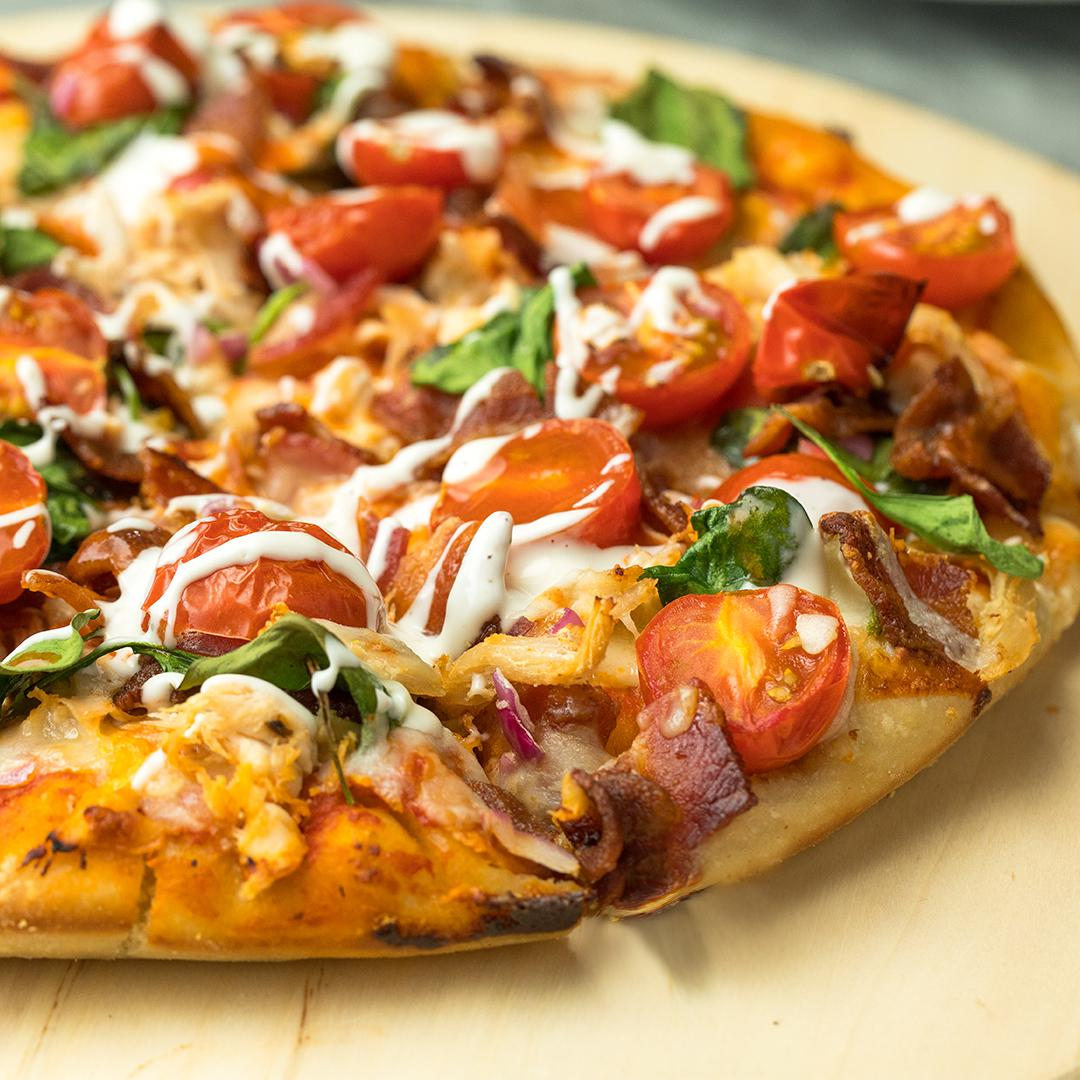
\includegraphics[width=1\textwidth,keepaspectratio]{../resources/pizza.jpg}
            \end{figure}
        \end{column}
    \end{columns}
\end{frame}

\begin{frame}
    \begin{columns}
        \begin{column}{0.5\textwidth}
            What am I not? 
            \begin{itemize}
                \item A sysadmin
                \item Good at making presentation slides
            \end{itemize}
        \end{column}
        \begin{column}{0.5\textwidth}
            \begin{figure}
                \centering
                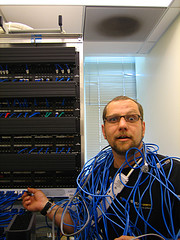
\includegraphics[width=1\textwidth,keepaspectratio]{../resources/sysadmin.jpg}
            \end{figure}
        \end{column}
    \end{columns}
\end{frame}

\begin{frame}
    \begin{columns}
        \begin{column}{0.5\textwidth}
            Does any of this matter?
            \begin{itemize}
                \item A sysadmin
                \item Good at making presentation slides
            \end{itemize}
        \end{column}
        \begin{column}{0.5\textwidth}
            \begin{figure}
                \centering
                
\includegraphics[width=1\textwidth,keepaspectratio]{../resources/nope.jpg}
            \end{figure}
        \end{column}
    \end{columns}
\end{frame}

\subsection{Home Networks eh?}

\begin{frame}
    \begin{columns}
        \begin{column}{0.5\textwidth}
            But why am I here presenting?
        \end{column}
        \begin{column}{0.5\textwidth}
            \begin{figure}
                \centering
                
\includegraphics[width=1\textwidth,keepaspectratio]{../resources/shrug.jpg}
            \end{figure}
        \end{column}
    \end{columns}
\end{frame}

\begin{frame}
    \begin{itemize}
        \item Home networks are fun
        \item Breaking your own stuff will assist in teaching you
        \item Can run some cool services for yourself/family/friends
    \end{itemize}
\end{frame}

\begin{frame}
    Am I going to be making any assumptions?
    \begin{itemize}
        \item We're not wanting to have a large number of "servers"
        \item We care about the security of our stuff
    \end{itemize}
\end{frame}

\begin{frame}
    \begin{columns}
        \begin{column}{0.5\textwidth}
            Are there reasons to not run a service on your home network?
        \end{column}
        \begin{column}{0.5\textwidth}
            \begin{figure}
                \centering
                
\includegraphics[width=1\textwidth,keepaspectratio]{../resources/confusion.jpg}
            \end{figure}
        \end{column}
    \end{columns}
\end{frame}

\section{Building A Home Network}
\subsection{What Might We Run?}

\begin{frame}
    \begin{columns}
        \begin{column}{0.5\textwidth}
            But I only want to run a few services...
        \end{column}
        \begin{column}{0.5\textwidth}
            \begin{figure}
                \centering
                
\includegraphics[width=1\textwidth,keepaspectratio]{../resources/logos.png}
            \end{figure}
        \end{column}
    \end{columns}
\end{frame}

\subsection{Moar Access, Moar Problems}

\begin{frame}
    \begin{columns}
        \begin{column}{0.5\textwidth}
            I want to be able to access my services from anywhere!
        \end{column}
        \begin{column}{0.5\textwidth}
            \begin{enumerate}
                \item Buy a domain, or use a freebie
                \item Pester your ISP for a static address (or big-brain it with some dynamic DNS)
                \item Setup some port forwards
                \item Done!
            \end{enumerate}
        \end{column}
    \end{columns}
\end{frame}

\begin{frame}
    Okay, cool, I have the things available on the interwebs...
\end{frame}


\begin{frame}
    \begin{columns}
        \begin{column}{0.5\textwidth}
            Should we leaving our applications in a default state?
        \end{column}
        \begin{column}{0.5\textwidth}
            \begin{figure}
                \centering
                
\includegraphics[width=1\textwidth,keepaspectratio]{../resources/oprah.png}
            \end{figure}
        \end{column}
    \end{columns}
\end{frame}

\subsection{Could We Secure Exposed Services Better?}

\begin{frame}
    \begin{columns}
        \begin{column}{0.5\textwidth}
            Nope! Let's apply some defence in depth! For simplicity in our setup I'd recommend SWAG
        \end{column}
        \begin{column}{0.5\textwidth}
            \begin{figure}
                \centering
                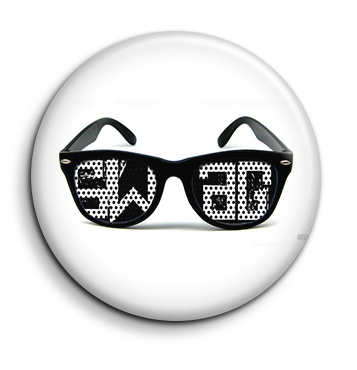
\includegraphics[width=1\textwidth,keepaspectratio]{../resources/wrong_swag.jpg}
            \end{figure}
        \end{column}
    \end{columns}
\end{frame}

\begin{frame}
    \begin{columns}
        \begin{column}{0.7\textwidth}
            This SWAG... \href{https://github.com/linuxserver/docker-swag}{https://github.com/linuxserver/docker-swag}
        \end{column}
        \begin{column}{0.3\textwidth}
            \begin{figure}
                \centering
                
\includegraphics[width=1\textwidth,keepaspectratio]{../resources/swag.png}
            \end{figure}
        \end{column}
    \end{columns}
\end{frame}

\begin{frame}
    Note: \textbf{SWAG is not required, it will just make your life easier in managing a reverse proxy}


    If you have the know-how of setting up a reverse proxy of your choosing, you could do so.

    \begin{figure}
        \centering
        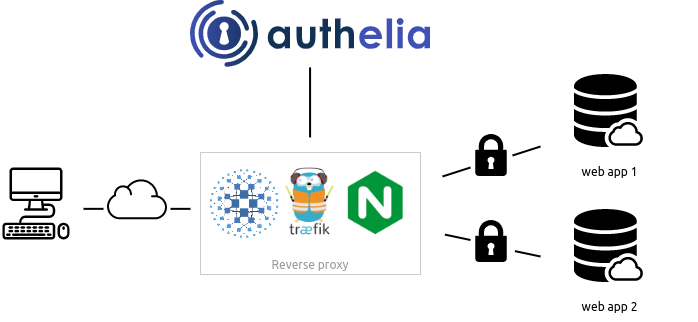
\includegraphics[width=1\textwidth,keepaspectratio]{../resources/archi.png}
    \end{figure}
\end{frame}

\end{document}